\documentclass{article}%
\usepackage[T1]{fontenc}%
\usepackage[utf8]{inputenc}%
\usepackage{lmodern}%
\usepackage{textcomp}%
\usepackage{lastpage}%
\usepackage{authblk}%
\usepackage{graphicx}%
%
\title{TspanC8 tetraspanins regulate ADAM10/Kuzbanian trafficking and promote Notch activation in flies and mammals}%
\author{Joseph Warren}%
\affil{Department of Bioengineering, University of California, Berkeley, California 94720, USA}%
\date{01{-}01{-}2005}%
%
\begin{document}%
\normalsize%
\maketitle%
\section{Abstract}%
\label{sec:Abstract}%
BASED ON DIGITAL PCR RESULTS\newline%
in order to experimentally characterize the function of red blood cells in T{-}cell classification.\newline%
such research could reduce cost, time, and healthcare in the United States.\newline%
the cost of the PCR test, produced and owned by this laboratory, and the time required to duplicate the results with help of SmartD, may be very favorable for many corporations.\newline%
in order to systematically discover the function of these cells in human marrowthe biologic foundation of cell divisionthereby helping to map out the human genome and early precursor disease processes, the platelet cell is a tremendous resource for this type of science\newline%
Red blood cells can be characterized from results of the PCR assay that may be compared with the factors that drive cell division. This study shows that the timing of cell differentiation can be improved. This improvement can greatly impact the efficiency of research programs in the field.\newline%
EDITORS NOTE: Caltech has supplied Stanfords Dr. Lynne Cox with a detailed annotated file on this research paper (p10, p26) and comments from Martin Zon/Stanfords Michael Hinton.

%
\subsection{Image Analysis}%
\label{subsec:ImageAnalysis}%


\begin{figure}[h!]%
\centering%
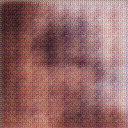
\includegraphics[width=150px]{500_fake_images/samples_5_427.png}%
\caption{A Black And White Photo Of A Black And White Striped Tie}%
\end{figure}

%
\end{document}